\documentclass[11pt]{article}
\usepackage{icmlko}
\begin{document}

\title{같은 개념, 다른 눈금 --- 공유 열에서는 그것이 다른 축이다}
\author{월드모델 실험실}
\date{노트 368 · 2026년 8월 1일}
\maketitle

\begin{abstract}
노트 365 · 366이 만화 258행 앞에 세운 벽을 헐러 갔다. 벽은
\texttt{media\_push} 채움이었다 --- 만든 스크립트가 없고, 읽는 쪽이 자리로
붙여 행이 늘면 축이 사라지고, 끄면 판이 $-0.0025$ 내려간다. \textbf{다시
만들었다.} 노트 108이 적어 둔 개념(``공식 외부 채널 수와 예고편 유무'')대로
AniList 에서 2,041건을 받아 저장소 안에 근거가 있는 눈금으로 채웠고, 읽는
쪽을 \textbf{id 기준}으로 고쳤다(아홉 번째 갈라진 목록이 닫혔다 --- 세계애니도
같이).

\textbf{개념은 맞았다} --- 새 값과 옛 값의 순위 상관이 \textbf{+0.9905},
라벨과의 연도 통제 상관이 $+0.4030$ 대 $+0.4080$ 으로 사실상 같다.
\textbf{그런데 판은 $-0.0029$(SD 0.0019, 1/12) 내려간다.} 갈라 보니
남은 차이는 \emph{눈금}뿐이었다 --- 옛 만화 값의 사분범위가 0.406 으로
\textbf{세계애니(0.546)와 맞춰져} 있는데 새 것은 0.250 으로 눌려 있다.
그리고 \textbf{제일 크게 다친 도메인이 세계애니($-0.0063$, 0/12)} 다 ---
\texttt{media\_push} 열을 같이 쓰는 바로 그 도메인이다.

\textbf{공유 열의 눈금은 그 열을 쓰는 도메인 전체에서 한 번 정해야 한다.}
도메인마다 따로 눈금을 매기면 한 열 안에 자가 둘 들어가고, 그것은 노트
357이 팝업 라벨에서 본 것과 같은 병이 \emph{피처 안에서} 나는 것이다.
안 넣었다. \textbf{그리고 노트 367의 새 폭이 첫 결정을 옳게 했다} ---
옛 폭이었으면 팝업 $+0.0188$(9/12)을 보고 \emph{더 나쁜 축을 채택}했을
것이다.
\end{abstract}

\section{벽을 헐었다}

\begin{itemize}
\item \textbf{다시 만들었다}(\texttt{ingest/manga\_push.py}). raw $=$ 외부
링크 수 $+$ (예고편 있으면 1), 값 $=$
\texttt{scale01(log2(raw+1), 0, 4)}. 눈금 관례는
\texttt{manga\_axes.venue\_prominence} 와 같은 것을 썼다 --- 저장소 안에
근거가 있는 눈금이다. 받은 분포: 외부 링크 중앙 3(분위 1·1·3·4·7·13) ·
예고편 24.9\%.
\item \textbf{배선을 id 로 고쳤다}(\texttt{state/tri\_domain.\_apply\_adopted}).
파일에 있던 \texttt{ids} 를 쓰고, 길이가 어긋나면 조용히 넘어가는 대신
\textbf{경고}를 남긴다. \textbf{세계애니도 같이 id 기준이 됐다} --- 노트
365가 ``그 도메인 행 수가 바뀌는 날 같은 일이 난다''고 지목한 덫이 닫혔다.
\end{itemize}

\section{개념은 맞았다}

\begin{center}
\begin{tabular}{lrr}
\hline
 & 옛 채움 & 새 채움 \\
\hline
순위 상관(공통 1,789행) & \multicolumn{2}{c}{$\mathbf{+0.9905}$} \\
라벨과 (연도 통제) & $+0.4080$ & $+0.4030$ \\
연도와 & $+0.2367$ & $+0.2162$ \\
옛 값 $\leftrightarrow$ 외부 링크 수 & \multicolumn{2}{c}{$+0.9523$} \\
옛 값 $\leftrightarrow$ 예고편 & \multicolumn{2}{c}{$+0.5935$} \\
\hline
\end{tabular}
\end{center}

노트 108의 주석 한 줄로 잃어버린 축을 되살릴 수 있었다. \textbf{개념을
적어 두는 것이 값을 했다.}

\section{그런데 판은 내려간다 --- 눈금 때문에}

\begin{center}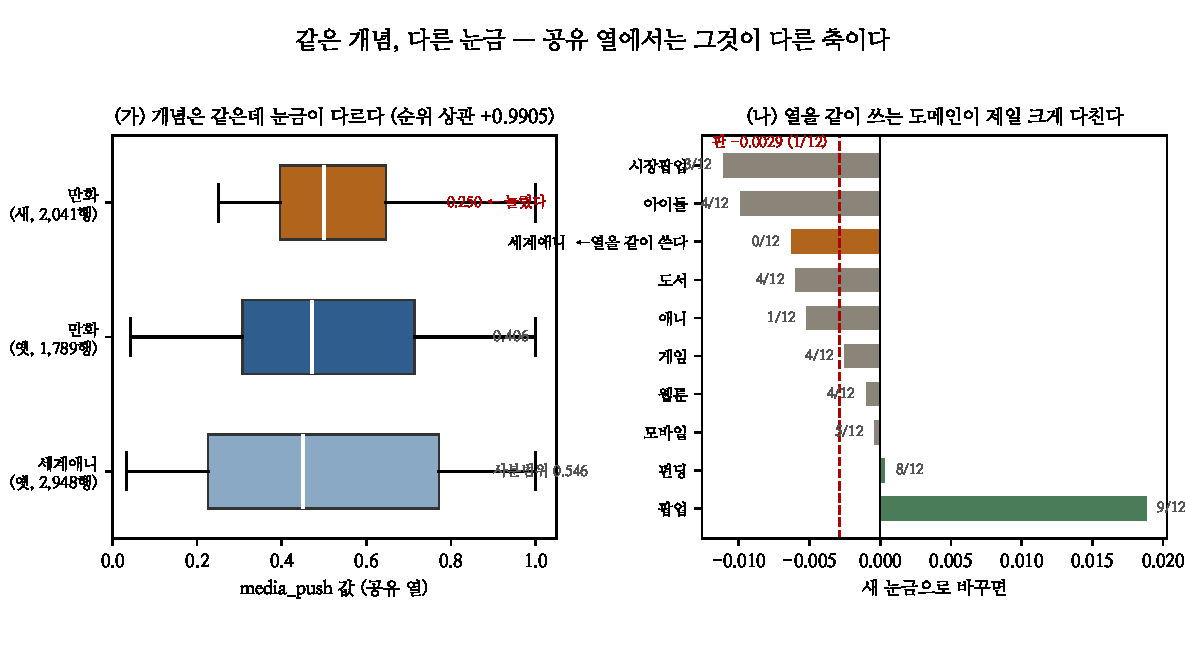
\includegraphics[width=\linewidth]{figs/scale.pdf}\end{center}

\begin{center}
\begin{tabular}{lrrr}
\hline
새 채움으로 바꾸면 & 차 & SD & 부호 \\
\hline
\textbf{판} & $-0.0029$ & 0.0019 & \textbf{1/12} \\
\textbf{세계애니} & $\mathbf{-0.0063}$ & 0.0023 & \textbf{0/12} \\
애니 & $-0.0052$ & 0.0037 & 1/12 \\
시장팝업 & $-0.0111$ & 0.0183 & 3/12 \\
팝업 & $+0.0188$ & 0.0321 & 9/12 \\
\hline
\end{tabular}
\end{center}

순위가 $+0.9905$ 로 같은데 판이 내려간다. 남은 차이는 \emph{눈금}뿐이다.

\begin{center}
\begin{tabular}{lrrr}
\hline
 & 중앙 & 사분범위 & 서로 다른 값 \\
\hline
세계애니 (옛) & 0.450 & 0.546 & 19 \\
만화 (옛)     & 0.472 & \textbf{0.406} & 21 \\
만화 (새)     & 0.500 & \textbf{0.250} & 16 \\
\hline
\end{tabular}
\end{center}

\textbf{옛 만화 값은 세계애니와 눈금이 맞춰져 있었다.} 사분범위 0.406 대
0.546 이고 중앙이 0.472 대 0.450 이다. 새 것은 $[0.25,\,0.75]$ 로 눌려
있다 --- $\log_2(n+1)$ 을 $[0,4]$ 로 자르는데 링크 수가 대개 1\textasciitilde{}13
이라 그 구간을 다 안 쓴다.

\textbf{그리고 제일 크게 다친 것이 세계애니다}($-0.0063$, \textbf{0/12}).
\texttt{media\_push} 는 \emph{공유 열}이고, 두 도메인의 값이 같은 열에
쌓인다. 만화 쪽 눈금을 누르면 그 열에서 세계애니의 값과 만화의 값이
서로 다른 자를 쓰게 되고, 나무가 그 열에서 가르는 자리가 어긋난다.

\textbf{노트 357이 팝업 라벨에서 본 것과 같은 병이다} --- 거기서는 계수
방법이 다른 두 자를 한 \emph{순위}에 넣었고, 여기서는 눈금이 다른 두 자를
한 \emph{열}에 넣는다. \textbf{같은 열에 두 자를 놓지 마라.}

\section{새 폭이 첫 결정을 옳게 했다}

노트 367이 미결정 폭을 고친 바로 다음 실험이다. 옛 규칙과 새 규칙이
반대 답을 낸다.

\begin{center}
\begin{tabular}{ll}
\hline
옛 규칙($\pm0.010$) & $|-0.0029| < 0.010$ $\Rightarrow$ 미결정 $\Rightarrow$
배포가 정함 $\Rightarrow$ 팝업 $+0.0188$(9/12) $\Rightarrow$ \textbf{채택} \\
새 규칙 & $|-0.0029| < 2{\times}$SD$(0.0039)$ 이나 부호 \textbf{1/12} 가
$[4,8]$ 밖 $\Rightarrow$ 판이 정함 $\Rightarrow$ \textbf{기각} \\
\hline
\end{tabular}
\end{center}

\textbf{옛 규칙이었으면 더 나쁜 축을 채택했다.} 새 폭이 한 번 쓰이자마자
값을 했다.

\section{안 넣는다 --- 그리고 무엇을 해야 하나}

옛 채움을 그대로 두고 id 배선만 살렸다(챔피언 0.4862 · 분모 2,723 확인).
새 채움은 \texttt{ingest/manga\_push.py} 로 남긴다.

\textbf{할 일이 정확해졌다: 눈금을 \emph{두 도메인에 걸쳐 한 번} 정한다.}
세계애니 2,948건의 외부 링크를 같이 받아, 만화 $+$ 세계애니를 합친
분포에서 백분위로 매기면 한 열에 자가 하나가 된다. 그러면 옛 채움을
버리고도 되고, 만화 258행도 같이 들어간다.

\section{규약에 더하는 줄}

\begin{itemize}
\item \textbf{공유 열의 눈금은 그 열을 쓰는 도메인 전체에서 한 번 정한다.}
도메인마다 따로 매기면 한 열에 자가 둘 들어간다.
\item \textbf{개념을 주석에 적어 두면 축을 되살릴 수 있다} --- 노트 108의
한 줄이 순위 $+0.9905$ 까지 복원해 줬다. \emph{스크립트는 사라져도 개념은
남는다.}
\item \textbf{채움은 id 로 붙이고, 못 붙이면 경고한다}(노트 365의 아홉 번째
갈라진 목록을 닫았다).
\end{itemize}

\section{남은 것}

\begin{center}
\begin{tabular}{ll}
\hline
갈래 & 지금 아는 것 \\
\hline
\textbf{눈금을 두 도메인에 걸쳐} & 세계애니 링크 2,948건 받아 합쳐 백분위. \\
 & 그러면 만화 258행이 따라 들어간다. \textbf{다음} \\
팝업 실측 41행 & 노트 360 · 364 · 366 \\
\hline
\end{tabular}
\end{center}

\end{document}
